% LuaLaTeX source; diagrams and data are embedded; myfont-setting.sty is required.
% Compile twice: lualatex easy-guide.tex
\documentclass[a4paper,11pt]{ltjsarticle}
\usepackage{myfont-setting}
\setmainjfont[BoldFont=HaranoAjiGothic-Bold.otf]{HaranoAjiMincho-Regular.otf}
\setsansjfont[BoldFont=HaranoAjiGothic-Bold.otf]{HaranoAjiGothic-Medium.otf}
\usepackage[margin=22mm,top=23mm,bottom=24mm]{geometry}
\usepackage{amsmath,amssymb,booktabs,longtable,array,tabularx}
\usepackage{graphicx,xcolor,tikz,pgfplots}
\usetikzlibrary{arrows.meta,positioning,calc,shapes.geometric}
\pgfplotsset{compat=1.18}
\usepackage{listings,enumitem,fancyhdr,tcolorbox,needspace}
\usepackage[section]{placeins}
\setcounter{tocdepth}{1}
\usepackage[unicode,hidelinks]{hyperref}
\definecolor{navy}{HTML}{254B63}
\definecolor{blue}{HTML}{447D9F}
\definecolor{orange}{HTML}{CF8153}
\definecolor{pale}{HTML}{F1F6F8}
\definecolor{graytext}{HTML}{586675}
\setlength{\parskip}{.38em}
\setlength{\emergencystretch}{2em}
\renewcommand{\arraystretch}{1.22}
\setlist{itemsep=.15em,topsep=.3em,leftmargin=1.7em}
\pagestyle{fancy}
\fancyhf{}
\fancyhead[L]{\small\sffamily Production Line Lab / 実装・実験・読み方}
\fancyhead[R]{\small v1.0.0}
\fancyfoot[C]{\thepage}
\setlength{\headheight}{16pt}
\lstset{basicstyle=\ttfamily\small,columns=fullflexible,keepspaces=true,
  breaklines=true,showstringspaces=false,frame=single,rulecolor=\color{blue!35},
  backgroundcolor=\color{pale},xleftmargin=.5em,xrightmargin=.5em,
  aboveskip=.7em,belowskip=.7em}
\DeclareRobustCommand{\code}[1]{\texttt{\detokenize{#1}}}
\pdfstringdefDisableCommands{\def\code#1{#1}}
\newcommand{\term}[1]{\textbf{#1}}
\newtcolorbox{pointbox}[1]{colback=pale,colframe=blue!70!black,title=#1,
  fonttitle=\bfseries,boxrule=.6pt,arc=1mm,left=2mm,right=2mm,top=1mm,bottom=1mm}
\newcolumntype{Y}{>{\raggedright\arraybackslash}X}
\newcolumntype{P}[1]{>{\raggedright\arraybackslash}p{#1}}
\tikzset{process/.style={draw=blue,fill=pale,rounded corners=2pt,
  minimum width=22mm,minimum height=9mm,align=center,font=\small},
  flow/.style={-{Stealth[length=2mm]},thick,draw=graytext}}

\begin{document}
\begin{titlepage}
\vspace*{12mm}
{\sffamily\color{blue}\Large 実装と実験の解説書}\par
\vspace{9mm}
{\sffamily\bfseries\Huge 生産ライン簡易デジタルツインによるボトルネック工程の定量抽出}\par
\vspace{9mm}
{\Large 工程エディタから、再現できるシミュレーションへ}\par
\vspace{8mm}
{\large 仕組み・操作・結果の説明}\par
\vfill
\vspace{7mm}
対象プログラム：\code{mock_line_editor.py}\par
版：1.0.0\quad 作成日：2026年9月21日\par
Hiroki Funashima
\vspace{4mm}
\end{titlepage}
\tableofcontents
\clearpage

\section{まず、何を作ったのか}
文化祭でサンドイッチを作る場面を考える。パンを焼く人、具を準備する人、
最後に組み立てる人がいる。具ができていても、パンがまだ焼けていなければ
組み立ては始められない。また、組立担当者が別の注文を作っていれば順番を待つ。
生産ラインでも、同じように「前の作業が終わるのを待つ」と「設備が空くのを待つ」が起きる。

今回のプログラムは、こうした順番と待ちを計算する実験装置である。
画面で作業工程を作り、その条件を保存し、製品を複数個流した場合の
開始時刻、終了時刻、待ち時間を求める。

\begin{pointbox}{完成した実装と、研究として残ること}
工程編集、JSON・CSV入出力、確率的な処理時間、分岐・合流を含む計算、
複数回試行、工程ランキング、図とCSVの出力を実装した。
一方、実工場で正しく予測できること、新しい学術的手法であること、
既存手法より優れていることは、今回の実装だけでは証明できない。
\end{pointbox}

\subsection{元のモックアップから変えた点}
元のプログラムは、画面と計算結果の表示をつなぐためのモックアップであった。
その計算は、出発点を一つ選び、次の工程も一つだけ選んで進んでいた。
さらに、待ち時間は設備の使用状況から求めず、乱数で作っていた。
そのため、元のグラフから実際のボトルネックを論じることはできなかった。

\begin{table}[htbp]\centering\small
\begin{tabularx}{\linewidth}{P{29mm}YY}
\toprule
項目 & 元のモックアップ & 今回の実装\\\midrule
製品の流れ & 一つの経路をたどる & 全製品が全工程を1回ずつ実行する\\
待ち時間 & 乱数で生成 & 前工程と設備の空きから算出する\\
分岐・合流 & 全枝の同期を扱わない & 並行作業とAND合流を扱う\\
設備台数 & 入力欄のみ & 同時に処理できる個数へ反映する\\
処理時間 & 定数・正規 & 定数・正規・一様・対数正規\\
保存 & 工程JSONの基本機能 & 工程・配置・実験条件のJSON保存と復元\\
評価 & 平均待ちの表示 & 設備待ち・合流待ち・稼働率・改善効果\\
再現性 & 固定seedによる仮計算 & seed・条件・コード指紋・ライブラリ版を記録\\
\bottomrule
\end{tabularx}
\caption{モックアップと実装版の対応。画面編集の基本的な操作を引き継いでいる。}
\end{table}

\Needspace{80mm}
\subsection{計画書の10タスクとの対応}
\begin{longtable}{P{9mm}P{47mm}P{92mm}}
\toprule No. & 計画書のタスク & 今回実装した内容\\\midrule\endhead
1 & 工程モデルの仕様 & 連結したDAG、AND分岐・合流、設備、投入条件を明記\\
2 & CSV入力形式 & \code{proc_time.csv}と\code{edges.csv}。12工程の直列・分岐例を同梱\\
3 & グラフと検査 & NetworkXで循環、孤立、分離、未定義接続、重複等を検査\\
4 & 処理時間生成 & 4分布、工程別の乱数系列、サンプル分布図\\
5 & ライン計算 & イベント駆動方式。製品・工程・設備別の時刻を出力\\
6 & 指標と順位 & 待ち時間、稼働率、各工程を短縮したときの全体改善量\\
7 & シナリオ & 4つの遅延工程設定と1つの対照条件\\
8 & 評価実験 & 各50試行、検出・誤検出・同率の集計。ばらつき等の12条件比較も追加\\
9 & 可視化 & ネットワーク、設備待ち、完了時間分布、改善効果、合流待ち、処理時間標本、時系列\\
10 & パッケージ & README、依存関係、サンプル、テスト、実行済み結果、本書\\
\bottomrule
\end{longtable}
計画書の「クリティカルパス寄与」などは指標の例である。
今回は待ちの発生場所を観察する指標と、工程改善の効果を直接比べる指標を採用した。
クリティカルパスの自動抽出は実装していない。
\clearpage

\section{計算する世界のルール}
\subsection{工程を点、順番を矢印で表す}
\term{ノード}は工程、\term{エッジ}は工程の順序関係を表す。
AからBへの矢印は「同じ製品について、Aの終了後にBが開始できる」という意味である。
矢印の向きをたどって元に戻らないグラフを\term{DAG（有向非巡回グラフ）}と呼ぶ。
今回、戻り作業や再加工は扱わない。

\begin{figure}[htbp]\centering
\begin{tikzpicture}[node distance=9mm and 17mm]
\node[process] (a) {A：パンを焼く};
\node[process,right=of a] (b) {B：仕上げ};
\node[process,below=of a] (c) {C：具を準備};
\node[process,right=of c] (d) {D：具の確認};
\node[process,right=of b,yshift=-9mm] (e) {E：組立};
\draw[flow] (a)--(b);\draw[flow] (c)--(d);
\draw[flow] (b)--(e);\draw[flow] (d)--(e);
\end{tikzpicture}
\caption{独立した準備を並行し、組立でそろうのを待つ例。EにはBとDの両方が必要である。}
\end{figure}

\subsection{分岐は「どちらも行う」、合流は「全部を待つ」}
分岐は、一つの製品に必要な複数の作業を並行して行うことを表す。
製品が確率的に右か左かの片方だけへ進む方式ではない。
合流では、同じ製品番号の前工程がすべて終了してから、設備待ちの列へ入る。
別の製品の部品を取り違えて組み合わせることはない。

製品は「完成させる注文・キット」と考えると分かりやすい。
枝に分かれても完成品が2個になるわけではない。
物理的な部品個数や原材料の消費を追う在庫シミュレーションではない。
枝が3本以上の分岐や、出発点・終点が複数ある連結DAGにも対応する。
完成条件は、その製品のすべての終点工程が終わったことである。

\subsection{設備と待ち行列}
各工程には専用の設備があり、初期値は1台である。
設備台数が2なら、同じ工程で2製品を同時に処理できる。
異なる工程の間で設備や作業員を共有することはない。

先に作業の準備が整った製品を先に処理する。
この方式を\term{FCFS（先着順）}という。
同じ時刻なら製品番号が小さいものを先にする。
同時刻に終了予定の処理と投入をまとめて反映し、それから空いた設備を割り当てる。
処理時間0の作業が生じた場合は、同じ時刻でさらに処理を進める。
この手順と、工程ID・設備番号の順序を固定し、同条件で順番が変わらないようにした。

\begin{table}[htbp]\centering\small
\begin{tabularx}{\linewidth}{P{36mm}Y}
\toprule 項目 & 仕様\\\midrule
待つ場所の広さ & 無制限。下流が満杯で上流が止まる現象は扱わない\\
搬送時間 & 0。必要なら搬送を専用工程として近似するが、その場合も設備モデルの仮定に従う\\
故障・休憩・段取り替え & なし\\
時刻0 & 全設備が空。製品がまだたまっていない状態から始める\\
製品数 & 指定個数を投入し、すべての完成まで計算する\\
単位 & 任意の共通時間単位。秒なら全入力を秒に統一する\\
処理時間の関係 & 異なる工程・製品・試行の処理時間は独立という仮定\\
途中の構造変更 & 1回の計算中は固定。実験と実験の間で編集する\\
\bottomrule\end{tabularx}
\caption{モデルの範囲。設備台数はモックアップの項目を動作させたもので、実験例はすべて1台である。}
\end{table}

\clearpage
\section{起動して、一度実験してみる}
\subsection{Linuxでの準備}
ZIPを展開し、\code{mock_line_editor.py}のあるフォルダへ移動する。
Python 3.12で動作を確認した。仮想環境を使うと、他の研究用プログラムのライブラリと分けて管理できる。
以下はUbuntuを想定したコマンドである。
\par\noindent\begin{minipage}{\linewidth}
\begin{lstlisting}
python3 -m venv .venv
source .venv/bin/activate
python -m pip install -r requirements.txt
python mock_line_editor.py
\end{lstlisting}
\end{minipage}\par
\code{venv}がないと表示された場合は、Ubuntuの\code{python3-venv}パッケージを導入する。
Qtの\code{xcb}関連エラーが出る環境では、エラーメッセージを確認し、
例えば不足している\code{libxcb-cursor0}などの実行時ライブラリを導入する。
今回の検証環境では画面を出さないQt実行も行ったが、通常利用では上の起動方法を使う。

\subsection{画面の見方と操作}
画面左は実験条件と選択工程の設定、右上は工程図、右下は結果である。
初期表示は12工程の分岐例である。
\begin{enumerate}
\item 工程をクリックし、工程名、分布、時間、設備台数を変更する。
\item 橙色の出力端子をクリックし、接続先の青い入力端子をクリックすると矢印ができる。
\item 工程はドラッグで移動できる。ホイールは拡大縮小、中ボタンのドラッグは表示位置の移動である。
\item 工程や矢印を選択してDeleteキー、または「選択削除」で削除する。工程削除では接続する矢印も消える。
\item 「工程追加」または右クリックのメニューから工程を追加できる。Escで接続操作を取り消せる。
\item 「JSON保存」で工程・配置・条件を保存する。
\item 「シミュレーション実行」で計算する。終了後に結果のタブを切り替える。
\item 「結果を保存」で、空のフォルダへCSV、JSON、PNG、PDFの図を出力する。
\end{enumerate}
循環する矢印、同じ矢印の重複、自分自身への接続は画面で追加できない。
直列例は横に長いため、全体表示では文字が小さくなる。必要な工程を拡大して編集する。

\subsection{実験条件の意味}
\begin{table}[htbp]\centering\small
\begin{tabularx}{\linewidth}{P{31mm}P{22mm}Y}
\toprule 項目 & 初期値 & 意味\\\midrule
製品数 & 60 & 1試行で完成させる注文の個数\\
試行回数 & 50 & 異なる乱数でライン全体を計算し直す回数\\
投入間隔 & 1 & 製品0を時刻0、製品1を時刻1、製品2を時刻2に投入\\
seed & 42 & 乱数の並びを決める整数。0〜$2^{32}-1$\\
短縮率 & 10\% & 各工程の処理時間を一つずつ10\%減らして比較する\\
改善比較 & 有効 & 基準計算に加え、各工程を変えた計算を行う\\
\bottomrule\end{tabularx}
\caption{初期条件。製品数と試行回数は1〜10,000、投入間隔は0以上。大きい設定では時間とメモリを多く使う。}
\end{table}
「60製品、50試行」は、1本のラインで3,000製品を連続生産する意味ではない。
空のラインから60製品を作る実験を、50回繰り返すという意味である。

改善比較は工程数を$V$、試行回数を$R$とすると、合計$R(V+1)$回のライン計算を行う。
12工程・50試行なら650回である。長い場合は「中止」で終了できる。
条件や工程を変更すると古いグラフを消すため、変更前の結果を新しい条件の結果と取り違えにくい。
計算中は工程編集を無効にし、別スレッドで計算する。

\clearpage
\section{工程のJSON保存と、変更後の再利用}
\subsection{何が保存されるか}
\code{JSON保存}には、工程ID、名前、処理時間の分布と数値、設備台数、接続、
画面の配置、実験条件が含まれる。
\code{JSON読込}で復元して、その続きを編集できる。
元のモックアップが保存したバージョン1のJSONも読み込める。
ただし、読込後の計算は今回のAND分岐・合流の仕様で行う。

接続を消して作り直す途中など、工程が分離している状態もJSONへ保存して再読込できる。
このような下書きは、接続を整えてから計算する。
一方、工程IDの重複、存在しない接続先、循環、不正な時間パラメータ等は拒否する。
読込に失敗した場合は、現在表示している工程を維持する。
未保存の状態でモデルを切り替える場合や終了する場合は、画面で確認する。

\subsection{小さなJSONの例}
次の例は、2工程を直列につないだ、そのまま読めるJSONである。
英語の項目名はプログラムが読むための固定名であり、変更しない。
\par\noindent\begin{minipage}{\linewidth}
\begin{lstlisting}
{
  "meta": {
    "version": 2,
    "semantics": "AND-fork-join/FCFS/unlimited-buffer"
  },
  "nodes": [
    {"id": "A", "name": "Cut", "capacity": 1,
     "service": {"dist": "constant", "p1": 2, "p2": 0}},
    {"id": "B", "name": "Assemble", "capacity": 1,
     "service": {"dist": "lognormal", "p1": 5, "p2": 1}}
  ],
  "edges": [{"id": "E1", "src": "A", "dst": "B"}],
  "layout": {"A": {"x": 0, "y": 0},
             "B": {"x": 210, "y": 0}},
  "simulation": {"jobs": 60, "runs": 50,
    "interval": 1, "seed": 42, "improvement": 0.1,
    "sensitivity": true, "all_traces": false}
}
\end{lstlisting}
\end{minipage}\par
\code{id}は工程を区別する番号、\code{name}は表示名である。
表示名は日本語にもできる。表示名の変更では乱数系列は変わらない。
工程IDは乱数系列にも使うため、同じ工程の比較を続ける場合には維持する。
画面はIDを自動付与する。IDそのものの変更はJSONまたはCSVで行い、矢印の参照も合わせる。

\subsection{変更前と変更後を混ぜない保存方法}
例えば\code{line_A_before.json}を保存した後で、工程を変更して
\code{line_A_after.json}へ保存する。結果も別フォルダへ出力する。
結果フォルダの\code{model.json}は、その計算に使った工程と条件のコピーである。
後で画面上の工程を変更しても、その結果フォルダの条件は変わらない。

結果の保存先が空でない場合は処理を止め、既存の実験結果を上書きしない。
JSON保存時の同名ファイルの置き換えは、ファイル選択画面の確認に従う。
自動保存や編集履歴をたどるUndo機能は実装していないため、区切りごとに名前を付けて保存する。

\clearpage
\section{CSVから工程を作る}
CSVは、表をカンマ区切りの文字で保存する形式である。
2つのファイルを同じフォルダに置く。文字コードはUTF-8を使う。
表計算ソフトで作る場合も、列名と工程IDを変えないよう注意する。

\subsection{工程の表}
\code{proc_time.csv}には次のように記載する。
\par\noindent\begin{minipage}{\linewidth}
\begin{lstlisting}
process,name,dist_type,p1,p2,capacity
A,Cut,constant,2,0,1
B,Assemble,lognormal,5,1,1
C,Inspect,uniform,1,3,1
\end{lstlisting}
\end{minipage}\par
必須列は\code{process,dist_type,p1,p2}である。
\code{name}を省略すると工程IDを名前とし、\code{capacity}を省略すると1台とする。
同じ工程IDを2行に記載してはいけない。

\subsection{接続の表}
\code{edges.csv}には次のように記載する。
\par\noindent\begin{minipage}{\linewidth}
\begin{lstlisting}
from,to
A,B
B,C
\end{lstlisting}
\end{minipage}\par
工程を追加するときは、工程表の行と、必要な接続の行を追加する。
削除するときは、その工程を参照する接続も削除する。
分岐は同じ\code{from}から複数行を、合流は同じ\code{to}へ複数行を記載する。
CSVには配置座標と実験条件を保存しない。読込時に配置を自動計算し、実験条件は画面で指定する。
これらも含めて残す場合はJSONを使う。

\clearpage
\section{処理時間のばらつきをどう表すか}
\subsection{平均と標準偏差}
処理時間が毎回必ず3秒なら定数でよい。
実際には2.8秒、3.1秒、3.4秒のように変化することがある。
平均は時間のおおよその中心、標準偏差は広がりの大きさを表す。
同じ平均3でも、標準偏差0.1と1.5では、短い作業や長い作業が出る程度が異なる。

\begin{table}[htbp]\centering\small
\begin{tabularx}{\linewidth}{P{25mm}P{29mm}P{29mm}Y}
\toprule 分布名 & p1 & p2 & 使う場面・注意\\\midrule
\code{constant} & 固定時間 $>0$ & 0 & 手計算による検証に向く\\
\code{normal} & 切上げ前の平均 $>0$ & 切上げ前の標準偏差 $\ge0$ & 左右に広がる正規乱数。負の値を0にする\\
\code{uniform} & 下限 $\ge0$ & 上限 $>$ 下限 & 範囲内の値を同じ密度で選ぶ\\
\code{lognormal} & 時間そのものの平均 $>0$ & 時間そのものの標準偏差 $\ge0$ & 正の時間で、右側に長い裾を持つ\\
\bottomrule\end{tabularx}
\caption{p1とp2の意味。分布によって意味が変わるため、同じ数値を機械的に流用しない。}
\end{table}

\subsection{正規分布で負の時間が出たら}
正規分布は負の値も取り得るが、作業時間が負になることはない。
実装は$X$を正規乱数として、$\max(0,X)$を使う。
これは「0未満が出たら引き直す」切断正規分布とは異なる。
0に値が集まり、実際の平均は入力した平均より大きくなる。
標準偏差が平均に比べて大きい場合、入力平均を実際の平均と思い込んではいけない。
ばらつきが大きい実験には、正の値を自然に生成する対数正規分布も用意した。

\subsection{対数正規分布の入力を分かりやすくした}
NumPyの対数正規乱数は、対数を取った後の平均・標準偏差を受け取る。
それを利用者に直接入力させると間違いやすいため、画面では元の時間の平均$m$と標準偏差$s$を入力する。
内部で
\[
 \sigma_{\log}^2=\log\left(1+\frac{s^2}{m^2}\right),\qquad
 \mu_{\log}=\log m-\frac{\sigma_{\log}^2}{2}
\]
へ変換する。式を覚える必要はない。「5秒、標準偏差1秒」と入力できることが大切である。

\subsection{seedと再現性}
コンピュータの乱数は、初期条件から計算で作る数列である。
今回、seed、試行番号、工程IDから工程別の乱数系列を作る。
工程IDはSHA-256という一定の規則で数へ変換し、NumPyの\code{SeedSequence}へ渡す\cite{numpy}。
Python標準の\code{hash()}は実行ごとに変わり得るため使っていない。

同じモデル、条件、seed、ライブラリ環境なら結果が再現する。
ファイルの工程記載順を入れ替えても乱数系列は変わらない。
異なるseedでの再確認も必要であり、「同じ数値が出る」と「仮定が現実に合っている」は別の問題である。
ライブラリ版や計算環境を変えたときの完全なビット単位の一致までは保証しない。

\clearpage
\section{時刻と待ち時間の計算を、手で確かめる}
\subsection{1台の設備に3製品が来る例}
処理に3秒かかる設備へ、時刻0、1、2に製品が来る。
最初の製品はすぐ始められるが、次の製品は前の製品の終了を待つ。
\begin{table}[htbp]\centering
\begin{tabular}{rrrrr}\toprule
製品番号 & 到着 & 開始 & 終了 & 設備待ち\\\midrule
0 & 0 & 0 & 3 & 0\\
1 & 1 & 3 & 6 & 2\\
2 & 2 & 6 & 9 & 4\\\bottomrule
\end{tabular}
\caption{平均待ち時間は$(0+2+4)/3=2$秒、全体完了時間は9秒である。}
\end{table}
設備待ちは乱数で作るのではなく、「開始−到着」で求める。
処理時間だけがばらつく場合、待ちはその結果として生まれる。

\subsection{合流で待つ例}
Aを2秒で処理し、その後Bは3秒、Cは7秒かかるとする。
BとCが終わると、Dで1秒かけて組み立てる。
Bは時刻5、Cは時刻9に終わるため、Dが開始できるのは時刻9である。
Dの設備が空いていれば、設備待ちは0、完成は時刻10となる。
しかし、先に終わったB側は4秒待っている。

\begin{figure}[htbp]\centering
\begin{tikzpicture}[x=1cm,y=.9cm]
\draw[->,graytext] (0,0)--(10.6,0) node[right]{時刻};
\foreach \x in {0,2,5,9,10}\draw (\x,.08)--(\x,-.08) node[below]{\x};
\foreach \y/\name in {1/D,2/C,3/B,4/A}\node[left] at (0,\y){\name};
\fill[blue!65] (0,3.75) rectangle (2,4.25);
\fill[blue!65] (2,2.75) rectangle (5,3.25);
\fill[blue!65] (2,1.75) rectangle (9,2.25);
\fill[orange!80] (9,.75) rectangle (10,1.25);
\draw[dashed,orange,thick] (5,3)--(9,3);
\node[above,font=\small] at (7,3.05){合流のため4秒待つ};
\draw[dotted] (9,0)--(9,3.2);
\end{tikzpicture}
\caption{合流待ちと設備待ちは別の原因で発生する。Dを速くしてもCの終了待ちは消えない。}
\end{figure}

\subsection{プログラムが記録する時刻}
製品$j$、工程$i$について、前工程がすべて終わった時刻を$R_{ji}$、
実際に開始した時刻を$S_{ji}$、終了時刻を$F_{ji}$、処理時間を$P_{ji}$とする。
\[
 R_{ji}=\max_{k\in\mathrm{Pred}(i)}F_{jk},\quad
 W_{ji}=S_{ji}-R_{ji},\quad
 F_{ji}=S_{ji}+P_{ji}.
\]
$\mathrm{Pred}(i)$は$i$の直前の工程の集合である。
出発工程には前工程がないので、$R_{ji}$を製品の投入時刻とする。
設備が空く順序と待ち行列を使って$S_{ji}$を決める。

合流待ちは、最初の前工程が終わってから最後の前工程が終わるまでの差
\[
 J_{ji}=R_{ji}-\min_{k\in\mathrm{Pred}(i)}F_{jk}
\]
と定義した。前工程が0個または1個なら0である。
これは「最初にできた部品が待った長さ」であり、すべての部品の待ち時間を足した量ではない。
同じ部品が複数工程の条件に使われることもあるため、全工程の$J$を足して
完成品の遅れそのものと解釈してはいけない。

\subsection{イベント駆動方式とは}
時計を0.001秒ずつ動かす代わりに、「次に製品が投入される時刻」や
「次に作業が終わる時刻」へ直接進む。
この方式を\term{離散事象シミュレーション}、またはイベント駆動方式と呼ぶ。
予定を時刻順に取り出すため、Python標準の\code{heapq}を使う\cite{heapq}。
これは予定表から最も早い予定を効率よく取り出す道具である。
時間を刻む幅に結果が左右される問題を避けられるが、計算機の小数の丸めは存在する。

\clearpage
\section{ボトルネックを何で判断するか}
\subsection{設備待ち：混雑のある場所}
工程$i$の平均設備待ちは、製品数を$N$として
\[
 \overline{W}_i=\frac{1}{N}\sum_{j=0}^{N-1}W_{ji}
\]
で求める。値が大きければ、その設備の前で長く待っている。
ただし、投入を速くしすぎれば、後工程の本当の制約にかかわらず先頭で待ちが増える。
また、上流の遅さによって下流には少しずつしか到着せず、下流の待ちが短くなることもある。

\subsection{稼働率：設備が使われていた割合}
全体完了時間を$T$、工程$i$の設備台数を$c_i$とすると
\[
 U_i=\frac{\sum_j P_{ji}}{c_i T}
\]
である。1に近ければ、観測期間を通じてほぼ使われ続けていた。
今回は空の状態から最後の完成までを分母に含めるため、立ち上がりや終了間際の空き時間も影響する。
有限個数の実験における稼働率であり、長期間安定運転したときの値ではない。

\subsection{改善効果：そこを速くすると全体は何秒短くなるか}
基準の全体完了時間を$T$とする。
工程$i$だけ処理時間を10\%短縮して計算し直した全体完了時間を$T_i^{(-10\%)}$として
\[
 \Delta_i=T-T_i^{(-10\%)}
\]
を求める。$\Delta_i$が大きい工程は、\term{この条件で10\%短縮すると効果が大きい改善候補}である。
待ち時間を直接減らしているわけではない。処理時間を変え、待ちを含めて全部計算し直す。

比較の前後で、同じ工程・同じ製品の処理時間標本を共有し、対象工程だけ0.9倍する。
これにより、別の乱数の偶然で速くなったのかという混乱を減らす。
標準偏差も0.9倍されるので、平均だけを減らして標準偏差を固定する介入ではない。

\begin{pointbox}{「改善候補」と「原因」の違い}
改善効果の順位は、投入間隔、製品数、短縮率、モデルの仮定に依存する。
順位1位が実工場の唯一の原因であるとは限らない。
設備を改善する費用も違うため、最大の短縮量が最も費用対効果のよい投資とは限らない。
\end{pointbox}

同率の最大値はすべて残す。数値上は絶対差$10^{-9}$、相対差$10^{-8}$の許容範囲を使う。
表示のための並び順と、統計的に順位が確定したことは別である。
小さな差、区間の重なり、複数の改善候補がある場合には、1位だけで判断しない。
工程を速くすると先着順の入れ替わりが起きる場合もあるため、負の$\Delta_i$も0に丸めず記録する。

\subsection{全体の指標}
\term{全体完了時間（makespan）}は、時刻0から全製品が完成するまでの長さである。
\term{平均滞在時間（mean flow）}は、各製品の「完成−投入」を平均した値である。
\term{生産率（throughput）}は$N/T$とする。秒なら単位は個/秒となる。
この値も、立ち上がりと終了を含む今回の有限ロットの平均である。

\clearpage
\section{結果ファイルとグラフの読み方}
\subsection{保存されるファイル}
\begin{longtable}{P{53mm}P{95mm}}
\toprule ファイル & 内容\\\midrule\endhead
\code{model.json} & 使用した工程・配置・実験条件。このJSONから再計算できる\\
\code{input_csv/} & 同じ工程をCSVの2表でも保存\\
\code{summary.json} & 全体・工程指標の平均、標準偏差、95\%区間\\
\code{runs.csv} & 各試行の完了時間、生産率、平均滞在時間\\
\code{node_metrics.csv} & 各試行・各工程の待ち、稼働率等\\
\code{trace.csv} & 製品・工程の投入、準備完了、開始、終了、設備番号等\\
\code{interventions.csv} & 各試行・各改善対象の基準時刻、変更後時刻、短縮量\\
\code{ranking.csv} & 改善効果順の工程表。改善比較を無効にしたときは待ち時間順\\
\code{reproducibility.json} & Python・ライブラリ版、コードのSHA-256、seed、保存対象範囲\\
\code{figures/} & 各図をPNGとPDFで保存\\
\bottomrule\end{longtable}
通常、\code{trace.csv}には基準条件の試行0だけを保存する。
巨大なファイルを避けつつ、時刻の詳しい確認ができるようにした。
全試行を保存する場合はCLIの\code{--all-traces}を指定する。
改善後の詳細時刻列は保存せず、改善後の全体完了時間を\code{interventions.csv}へ残す。

\begin{table}[htbp]\centering\small
\begin{tabularx}{\linewidth}{P{35mm}Y}
\toprule traceの列 & 意味\\\midrule
\code{run,job,process} & 試行番号、製品番号、工程ID。番号は0から始まる\\
\code{server} & 工程内の設備番号。0から始まる\\
\code{release} & 製品の投入時刻\\
\code{first_component} & 前工程のうち最初に終わった時刻。出発工程では投入時刻\\
\code{ready} & 前工程がすべて終了し、設備待ち列へ入った時刻\\
\code{start,finish} & 実際の開始と終了\\
\code{service} & 実際に使った処理時間標本\\
\code{queue_wait} & \code{start-ready}\\
\code{sync_wait} & \code{ready-first_component}\\
\bottomrule\end{tabularx}
\caption{時刻表の列。工程をまたぐ先後関係や同じ設備の処理重複を確認できる。}
\end{table}
\code{queue_total}は全製品の設備待ち合計、\code{queue_mean}は1製品あたりの平均である。\par
\code{queue_time_average}は\code{queue_total}/$T$で、待ち列の長さを時間で平均した値である。
平均の単位がそれぞれ違うことに注意する。
\code{ranking.csv}の\code{queue_mean_mean}は「各試行の製品平均を、さらに試行間で平均した値」を表す。

\subsection{棒グラフと95\%区間}
棒は各試行の値を平均したものである。図の細い線は平均値の95\%信頼区間を表す。
試行回数$R$、試行間の標準偏差$s$に対して
\[
 \overline{x}\ \pm\ t_{0.975,R-1}\frac{s}{\sqrt R}
\]
を使う。係数$t$はSciPyで求める\cite{scipy}。
同じ手順で実験を何度もやり直して区間を作ると、条件を満たす場合に、その約95\%が
仮想モデルの平均値を含む、という意味である。
全製品の95\%がこの範囲に入るという意味ではない。

設備待ち等は1試行内で製品間の依存があるため、独立な標本の単位を「製品」ではなく「試行」とする。
改善効果は、各試行の差$\Delta_i$を作った後で区間を求める。
試行1回では区間を出さず、JSONでは\code{null}、CSVでは空欄になる。
歪みが強い分布や少ない試行数では、この区間の近似は十分でない場合がある。
工程ごとの区間であり、多数の工程を同時に判定するための補正はしていない。

\subsection{それぞれの図で見るもの}
\begin{itemize}
\item \code{network}：順序関係。橙色は平均改善効果が最大の工程。
\item \code{queue_wait}：設備の前の混雑。原因そのものとは限らない。
\item \code{join_wait}：枝の完了時刻がどの程度ずれるか。
\item \code{makespan}：試行ごとの全体完了時間の分布。
\item \code{improvement}：各工程を個別に短縮した場合の全体改善量。
\item \code{service_samples}：試行0で生成した処理時間。理論分布そのものではなく有限個の標本。
\item \code{timeline}：試行0の最初の8製品の処理区間。色は製品番号。同一工程で設備が複数あると棒が重なり得るため、設備別確認にはCSVを使う。
\end{itemize}
PNGはスライドへ貼りやすく、PDFの図は拡大しても線が滑らかである。
保存図では工程IDをラベルにし、フォント環境による日本語の文字化けを避けた。
工程名との対応は\code{ranking.csv}と\code{model.json}にある。

\clearpage
\section{実際に行った検証実験}
\subsection{プログラムがルール通りに動くか}
自動テストは27件すべて通過した。
特に、1台の設備の待ち時間、2台設備、直列の手計算、分岐・合流、
複数の出発点・終点、処理時間0、工程間の先後関係、設備使用の非重複、
JSON・CSVの保存復元、同一seedの再現性、不正入力を確認した。
直列ラインではイベント方式と独立な漸化式を用い、ランダムな処理時間行列で時刻を照合した。
GUIの工程選択だけで値が書き換わらないこと、工程削除とデータの一致も確認した。

さらに、画面を出さないQt環境で実際にGUIを起動し、バックグラウンド計算から
結果表示までを確認して画面画像を保存した。
これは手元のUbuntu・Wayland環境で全操作を実測したことを意味しない。
テスト成功は、確認した条件で実装が仕様に合うことの証拠であり、すべての入力や現実への適合の証明ではない。

\subsection{12工程のラインと5つのシナリオ}
直列例はN01からN12まで順番に進む。
分岐例ではN02の後でN03--N05とN06--N08へ分かれ、N09で合流する。
前後を含めた工程数はいずれも12である。
\begin{figure}[htbp]\centering
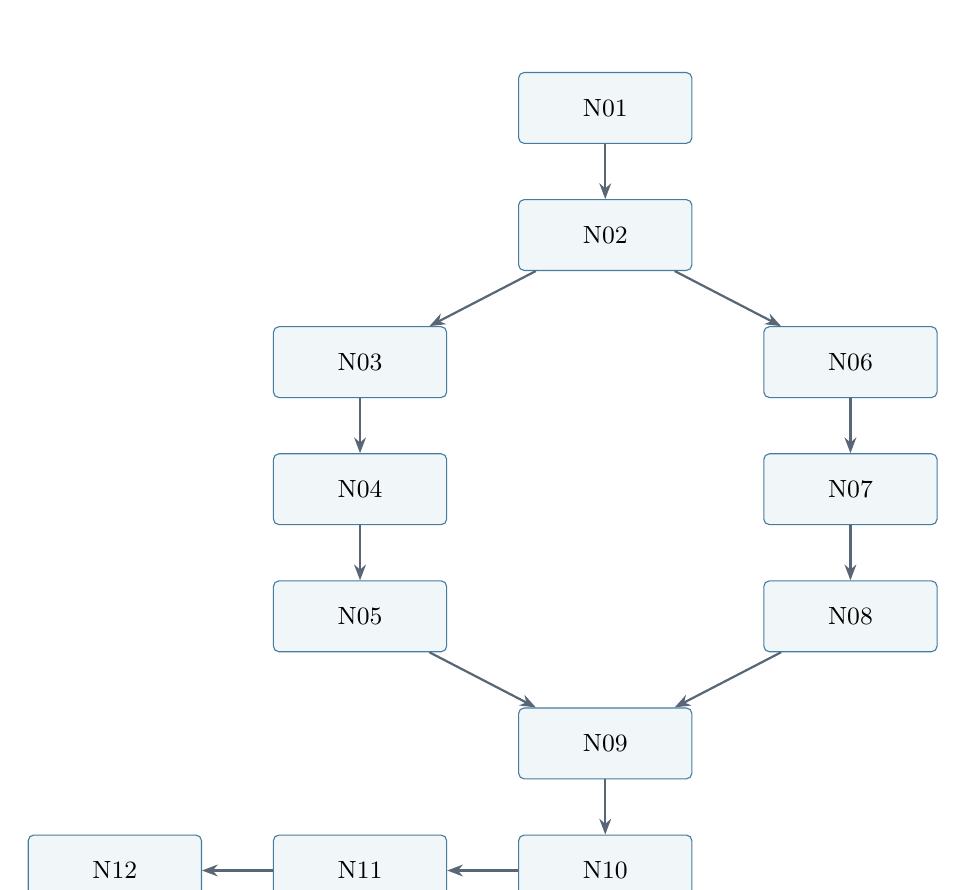
\begin{tikzpicture}[node distance=7mm and 9mm]
\node[process] (n01) {N01};
\node[process,below=of n01] (n02) {N02};
\node[process,below left=of n02] (n03) {N03};
\node[process,below right=of n02] (n06) {N06};
\node[process,below=of n03] (n04) {N04};
\node[process,below=of n06] (n07) {N07};
\node[process,below=of n04] (n05) {N05};
\node[process,below=of n07] (n08) {N08};
\node[process,below right=of n05] (n09) {N09};
\node[process,below=of n09] (n10) {N10};
\node[process,left=of n10] (n11) {N11};
\node[process,left=of n11] (n12) {N12};
\foreach \a/\b in {n01/n02,n02/n03,n02/n06,n03/n04,n04/n05,n06/n07,n07/n08,n05/n09,n08/n09,n09/n10,n10/n11,n11/n12}
\draw[flow] (\a)--(\b);
\end{tikzpicture}
\caption{分岐モデルの接続。画面上の座標は計算結果に影響しない。矢印が順序を決める。}
\end{figure}

\begin{table}[htbp]\centering\small
\begin{tabularx}{\linewidth}{P{29mm}P{20mm}P{19mm}Y}
\toprule シナリオ & 変更工程 & 期待する工程 & 条件\\\midrule
直列・中間 & N06 & N06 & N06の平均を3から4.5へ\\
直列・先頭 & N01 & N01 & N01の平均を3から4.5へ\\
分岐・枝 & N06 & N06 & N06の平均を3から4.5へ\\
分岐・合流 & N09 & N09 & N09の平均を3から4.5へ\\
対照条件 & N03 & N06 & N03を1から1.5へ。N06は8で据え置く\\
\bottomrule\end{tabularx}
\caption{先に定めた評価条件。「変更した工程」と「ボトルネックとして期待する工程」を分ける。}
\end{table}
最初の4条件は正規分布で、通常工程は平均3・標準偏差0.45とする。
対象工程は両方を1.5倍し、平均4.5・標準偏差0.675とした。
つまり平均だけを上げた実験ではなく、標準偏差/平均の比を一定にした遅延設定である。
対照条件はすべて定数で、N06が8、変更後N03が1.5、その他は2とした。

全条件で、60製品、50試行、投入間隔1、seed 42、設備1台、改善時の処理時間短縮率10\%を使った。
期待工程は設計上のラベルであり、確率的な各試行の「唯一の真の原因」を外部測定したものではない。
特に変動が大きいときには、実際に効く工程が試行ごとに変わり得る。

\subsection{検出率と誤検出}
各試行で、指標が最大の工程を選ぶ。唯一の最大工程が期待工程と一致した回数を正検出とする。
別の工程なら誤検出、複数工程が同率なら曖昧とする。
\code{detection_summary.csv}に3つを分けて記録し、
\code{confusion.csv}には期待工程と選ばれた工程の組を集計する。

\begin{table}[htbp]\centering
\begin{tabular}{lrrr}\toprule
シナリオ & 設備待ち & 稼働率 & 改善効果\\\midrule
直列・中間 & 0/50 & 50/50 & 50/50\\
直列・先頭 & 50/50 & 50/50 & 50/50\\
分岐・枝 & 0/50 & 50/50 & 50/50\\
分岐・合流 & 0/50 & 50/50 & 50/50\\
対照条件（定数） & 50/50 & 50/50 & 50/50\\\bottomrule
\end{tabular}
\caption{期待工程と唯一の1位が一致した回数。同率はこの実験では0件。確率条件の0/50は50回とも別の工程を選んだ。}
\end{table}
確率条件で50/50のとき、Wilson法による検出確率の95\%区間は約92.9〜100\%である。
0/50のときは約0〜7.1\%となる。
50回成功したから成功確率100\%が証明された、とは言えない。
対照条件は同じ計算を50回繰り返しているため、50個の独立した確率的な証拠とはみなさず、
検出率の確率的な区間は出さない。
また、条件間では同じ乱数を共有するため、5条件を単純に足して独立な250試行とは扱わない。

\begin{pointbox}{この結果から言える重要な点}
この5条件では、改善効果と稼働率が同じ期待工程を抽出した。
したがって、改善効果の指標が稼働率より優れているという実験結果にはなっていない。
一方、設備待ちだけでは誤る設定が存在することを、具体的に確認できた。
\end{pointbox}

\subsection{待ちが最大でも、改善効果が最大とは限らない}
直列・中間の例では、N01の平均設備待ちは58.76、N06は38.71であった。
投入間隔が1であるのに、最初の工程に平均3かかるため、入口から列が伸びる。
ところがN01を10\%速くしても、N06の平均4.5が全体の流れを制限し続ける。
\begin{table}[htbp]\centering
\begin{tabular}{lrrr}\toprule
工程 & 平均設備待ち & 平均稼働率 & 平均短縮時間［95\%区間］\\\midrule
N01 & 58.76 & 0.591 & 0.321［0.292, 0.351］\\
N06 & 38.71 & 0.891 & 26.761［26.580, 26.941］\\
N09 & 0.047 & 0.591 & 0.311［0.295, 0.328］\\\bottomrule
\end{tabular}
\caption{直列・中間の実行結果。待つ場所と、全体を速くできる場所の違いが大きい。単位は共通の仮想時間単位。}
\end{table}

\begin{figure}[p]\centering
\begin{tikzpicture}
\begin{axis}[width=.94\linewidth,height=57mm,ybar,bar width=5mm,
  symbolic x coords={N01,N02,N03,N04,N05,N06,N07,N08,N09,N10,N11,N12},xtick=data,x tick label style={font=\scriptsize,rotate=30,anchor=east},
  ylabel={平均設備待ち},title={設備の前で待つ時間},ymin=0,grid=major,grid style={gray!15},
  tick label style={font=\small},title style={font=\small},
  error bars/y dir=both,error bars/y explicit]
\addplot+[fill=blue!75,draw=blue,error bars/error bar style={black},error bars/error mark options={black}]
 coordinates {(N01,58.758557) +- (0,0.612426) (N02,2.457342) +- (0,0.493761) (N03,1.483787) +- (0,0.234930) (N04,1.284073) +- (0,0.209834) (N05,0.979293) +- (0,0.221528) (N06,38.705111) +- (0,0.839215) (N07,0.007165) +- (0,0.002320) (N08,0.028774) +- (0,0.006241) (N09,0.047063) +- (0,0.006731) (N10,0.056942) +- (0,0.008150) (N11,0.061089) +- (0,0.006790) (N12,0.068481) +- (0,0.009631)};
\end{axis}
\end{tikzpicture}

\begin{tikzpicture}
\begin{axis}[width=.94\linewidth,height=57mm,ybar,bar width=5mm,
  symbolic x coords={N01,N02,N03,N04,N05,N06,N07,N08,N09,N10,N11,N12},xtick=data,x tick label style={font=\scriptsize,rotate=30,anchor=east},
  ylabel={全体完了時間の短縮},title={その工程を10\%短縮したときの効果},ymin=0,grid=major,grid style={gray!15},
  tick label style={font=\small},title style={font=\small},
  error bars/y dir=both,error bars/y explicit]
\addplot+[fill=orange!75,draw=orange,error bars/error bar style={black},error bars/error mark options={black}]
 coordinates {(N01,0.321213) +- (0,0.029523) (N02,0.320065) +- (0,0.026148) (N03,0.313212) +- (0,0.020818) (N04,0.311888) +- (0,0.013536) (N05,0.311280) +- (0,0.011434) (N06,26.760514) +- (0,0.180307) (N07,0.306772) +- (0,0.013027) (N08,0.313159) +- (0,0.020538) (N09,0.311259) +- (0,0.016522) (N10,0.308917) +- (0,0.018808) (N11,0.320068) +- (0,0.018647) (N12,0.323588) +- (0,0.032825)};
\end{axis}
\end{tikzpicture}

\caption{直列・中間の50試行。上は設備待ち、下は改善効果。細い線は試行間の平均の95\%区間である。N01の待ちが最大でも、N06を速くする効果の方が大きい。}\end{figure}
\begin{figure}[htbp]\centering
\begin{tikzpicture}
\begin{axis}[width=.8\linewidth,height=55mm,ybar,bar width=11mm,ymin=0,
  xlabel={全体完了時間},ylabel={試行数},grid=major,grid style={gray!15}]
\addplot[fill=blue!70,draw=white] coordinates {(296.465442,5) (299.704907,11) (302.944373,16) (306.183838,5) (309.423303,10) (312.662769,2) (315.902234,1)};
\end{axis}\end{tikzpicture}
\caption{直列・中間の完了時間の分布。50回の実験結果を7区間に分けた。単一の完了時間だけで判断せず、ばらつきも確認する。}
\end{figure}

基準の全体完了時間の平均は303.896、平均の95\%区間は302.530〜305.261である。
N06の処理時間を10\%短縮すると、全体は平均で約26.76短くなった。
「工程が10\%速い」からといって、全体も必ず10\%短くなるわけではない。

分岐・枝の例では、合流工程N09の合流待ちは平均40.04あったが、
N09自体を速くする効果は約0.311にとどまった。
N06を速くする効果は約26.84であり、合流に到着するのを待っている理由を見分ける必要がある。

\subsection{変えた工程がボトルネックとは限らない}
対照条件ではN03を1から1.5へ遅くしたが、N06には8かかっていた。
N03を10\%速くしても全体短縮は0、N06を10\%速くすると48短くなった。
全体完了時間は496から448になった。
遅くした場所を無条件に正解ラベルにすると、評価の考え方自体を誤ることが分かる。

\clearpage
\section{ばらつきと投入間隔を変える追加実験}
平均だけではなく、処理時間のばらつきによって列の様子が変わる。
そこで、直列と分岐の2種類、投入間隔1と5の2種類、ばらつきの3段階を組み合わせ、12条件を計算した。
\code{variance_sweep.py}で再現できる。

ばらつきは\term{変動係数（CV）}で指定する。
\[
 \mathrm{CV}=\frac{\text{標準偏差}}{\text{平均}}
\]
例えば平均3、CV 0.5なら標準偏差は1.5である。
この実験では、対数正規分布を使い、N06の平均を4.5、他を3に固定した。
CVは0、0.15、0.5、製品数60、試行50、seed 42、短縮率10\%である。
CV 0では処理時間が毎回同じになる。

\begin{table}[htbp]\centering\small
\begin{tabular}{lrrrrr}\toprule
構造 & 投入間隔 & CV & 全体完了時間 & N06の設備待ち & N06の改善効果\\\midrule
直列 & 1 & 0 & 303.00 & 44.25 & 27.00 \\
直列 & 1 & 0.15 & 303.79 & 38.55 & 26.75 \\
直列 & 1 & 0.5 & 314.63 & 28.14 & 20.95 \\
直列 & 5 & 0 & 332.50 & 0.00 & 0.45 \\
直列 & 5 & 0.15 & 333.27 & 0.68 & 0.84 \\
直列 & 5 & 0.5 & 345.96 & 5.09 & 3.99 \\
分岐 & 1 & 0 & 294.00 & 44.25 & 27.00 \\
分岐 & 1 & 0.15 & 294.56 & 42.17 & 26.83 \\
分岐 & 1 & 0.5 & 302.74 & 38.92 & 22.83 \\
分岐 & 5 & 0 & 323.50 & 0.00 & 0.45 \\
分岐 & 5 & 0.15 & 323.85 & 0.42 & 0.71 \\
分岐 & 5 & 0.5 & 333.86 & 4.41 & 3.69 \\
\bottomrule\end{tabular}
\caption{12条件の実行結果。値は50試行の平均。詳細な95\%区間は\code{variance_summary.csv}に保存している。全条件で平均改善効果の最大はN06であった。}\end{table}

投入間隔1では、N06の平均が4.5のため、次々と製品がたまる。
直列でCV 0から0.5へ変えると、全体完了時間は303.00から314.63へ増えた一方、
N06の設備待ちは44.25から28.14へ減った。上流のばらつきで到着も不規則になり、
「全体が遅くなるのに、ある場所の待ちは減る」という結果も起こる。

投入間隔5では到着が遅くなるため、CV 0なら設備待ちは全工程0である。
N06を10\%速くしても短縮は0.45にとどまる。
同じ直列モデルでも、投入間隔1では27.00短縮できた。
CV 0.5では時々長い処理が発生して待ちが生じ、投入間隔5でもN06の改善効果が約3.99となった。

投入間隔5の全体完了時間が投入間隔1より長いのは、最後の製品を投入する時刻自体が遅いからである。
それだけを見て「ラインの設備が悪くなった」と判断してはいけない。
投入間隔の比較では、生産の予定、設備待ち、製品の滞在時間を合わせて読む。


この比較は有限ロット、無制限待ち場所、独立な処理時間という仮定の下での探索的な実験である。
条件を変えたときの変化を観察する用途に向く。
CVを大きくすれば、どんなラインでも必ず同じ割合で悪化する、という一般法則を示したものではない。
CV 0の反復は全く同じ結果になるため、繰返し回数を増やしても新しい情報は増えない。

\clearpage
\section{プログラムの中身を読む}
\subsection{1ファイルの中を9つの役割に分けた}
本体は\code{mock_line_editor.py}という1つのファイルである。
配布を簡単にするため1ファイルを保ちながら、データ、計算、入出力、画面を節ごとに分けた。
画面を使わないCLIでも同じ計算関数を呼ぶため、別の計算方法へ分かれない。

\begin{table}[htbp]\centering\small
\begin{tabularx}{\linewidth}{P{42mm}Y}
\toprule クラス・関数 & 役割\\\midrule
\code{ServiceSpec} & 分布名とp1・p2をひとまとまりのデータにする\\
\code{NodeSpec,EdgeSpec} & 工程と接続の情報を表す\\
\code{LineModel} & 全工程、接続、配置。検証とJSON用データへの変換\\
\code{SimulationConfig} & 製品数、試行数、seedなどの計算条件\\
\code{load_json,load_csv} & ファイルを読み、形式と整合性を確認する\\
\code{draw_services} & 工程別・試行別に処理時間の表を生成する\\
\code{Simulator.run} & 1試行分の設備、待ち列、イベントを動かす\\
\code{RunResult} & 1試行の結果をひとまとまりにする\\
\code{run_experiment} & 複数回試行と工程別改善実験を行う\\
\code{ExperimentResult} & 基準計算、改善結果、集計、時刻表をまとめる\\
\code{export_result} & 使用モデル、条件、CSV、統計、環境情報を出す\\
\code{export_figures} & 保存する図を作る\\
\code{run_benchmark} & 5シナリオの期待工程との一致を集計する\\
\code{build_gui_classes} & 必要なときだけQtを読み込み、画面用クラスを定義する\\
\code{main} & 起動方法を読み、GUIまたはCLIを実行する\\
\bottomrule\end{tabularx}
\caption{本体の構造。\code{dataclass}は関連する値に名前を付けてまとめるPythonの仕組みである。}
\end{table}

\begin{figure}[htbp]\centering
\begin{tikzpicture}[node distance=11mm and 11mm]
\node[process] (json) {JSON / CSV};
\node[process,right=of json] (model) {工程データ\\検査};
\node[process,right=of model] (calc) {時刻計算\\改善比較};
\node[process,below=of calc] (stats) {統計・図・CSV};
\node[process,below=of model] (gui) {画面編集};
\draw[flow] (json)--(model);\draw[flow] (model)--(calc);\draw[flow] (calc)--(stats);
\draw[flow] (gui)--(model);\draw[flow] (model)--(json);
\end{tikzpicture}
\caption{データの流れ。画面の座標や色は計算の入力条件にはならない。}
\end{figure}

\subsection{GUIの担当}
\code{EditorScene}が工程図とそのデータを管理し、\code{NodeItem}と\code{EdgeItem}が
見た目を担当する。\code{PropertyPanel}は選択工程の数値を編集する。
\code{MainWindow}がファイル操作、実行、表示をつなぐ。
\code{Worker}は\code{QThread}を使い、計算中も画面が応答できるようにする。
実行時には工程データをコピーして計算へ渡す。

元の実装では、工程を選び直して入力欄へ値を表示するだけでも変更通知が出るため、
別工程のパラメータで値を上書きする危険があった。
今回、表示を設定している間は更新通知を抑えた。
さらに、右クリックでの追加や工程削除も、画面と内部データが一致するように整理した。

\subsection{計算時間とメモリの目安}
$N$製品、$V$工程なら、基本となる処理時間・開始・終了等の表は$N\times V$の大きさになる。
イベントは主として製品投入と各工程の終了で発生する。
実装はイベント時刻ごとに各工程の待ち列を確認するため、単にノード数だけで速度は決まらない。
改善比較は工程数に応じて計算回数が増える。

対象は計画書通り10〜30工程程度である。例は12工程であり、入力で10〜30に固定はしていない。
大量の工程・製品・全試行時刻表を同時に使う場合は、より大きなメモリが必要になる。
複数コアで試行を並列計算する機能はない。GUI用スレッドは画面の応答を保つためである。

\clearpage
\section{使用したライブラリ}
\begin{longtable}{P{25mm}P{19mm}P{105mm}}
\toprule 名前 & 検証時の版 & 何を担当するか\\\midrule\endhead
NumPy & 2.3.5 & 多数の数値を表として扱い、処理時間の乱数を作る\\
NetworkX & 3.7 & 矢印つきグラフを作り、DAG・連結性・工程順を調べる\\
SciPy & 1.17.0 & 平均の信頼区間に使うStudentの$t$分布\\
Matplotlib & 3.10.8 & 発表資料に使えるPNG・PDFの図を保存\\
PyQt6 & 6.11.0 & ウィンドウ、工程図、入力欄、ファイル操作、別スレッド計算\\
PyQtGraph & 0.14.0 & GUI内で結果のグラフを表示\\
pytest & 9.1.1 & 手計算との一致、入力検証、保存復元などの自動テスト\\
\bottomrule\end{longtable}
Pythonは3.12.14で確認した。標準ライブラリの\code{dataclasses}、\code{json}、
\code{csv}、\code{heapq}、\code{hashlib}、\code{argparse}、\code{pathlib}なども使う。
標準ライブラリはPythonに含まれるため別途インストールしない。

NetworkXのDAG用関数は、すべてが自動で循環を検査するわけではないので、
本プログラムで事前に明示的な検査を行う\cite{networkx}。
PyQtの通知機構を用いて、計算終了を画面に伝える\cite{pyqt}。
SimPyは今回の依存関係には含めていない。待ち行列とイベント処理を、学習のため本体内に実装した。

\clearpage
\section{現在、何が言えて、何が問題か}
\subsection{現時点で言えること}
\begin{enumerate}
\item 今回定義した仮想ラインのルールに基づき、複数製品の時刻と待ちを計算できる。
\item 工程と条件をJSONへ保存し、工程を変更した後も以前の条件を復元して実験できる。
\item 手計算や独立な直列計算と一致し、検証した入出力と画面操作は動作した。
\item 入力過多のラインでは、平均設備待ちの最大工程と改善効果の最大工程が一致しない例がある。
\item 既定の5シナリオでは、改善効果の順位が期待した工程を選んだ。ただし稼働率でも同じ結果となった。
\item 条件を変える実験によって、工程の構造、ばらつき、投入間隔の影響を数値で調べられる。
\end{enumerate}

\subsection{実工場のデジタルツインと呼べるか}
今回の実装には、実工場のセンサーとの接続、現物の状態を取り込む更新、
実測データによるパラメータ調整がない。
NISTが説明するデジタルツインの重要な要素には、物理的な対象との接続・同期が含まれる\cite{nist}。
したがって本成果物の実態は、\term{生産ラインの簡易シミュレータ、またはデジタルツインへ進むための試作}と表すのが適切である。
名称だけで現実との対応が保証されるわけではない。

\subsection{計画書の新規性の主張は、まだ検証が必要である}
工程をグラフで表すこと、確率的な処理時間を使うこと、待ち行列を計算すること、
ボトルネックを指標で比較すること自体には、既存の研究や方法がある。
例えばWestらは、動的ボトルネックの診断指標を提案し、離散事象シミュレーションの9シナリオで評価している\cite{west}。
そのため計画書の「客観的指標による手法は十分に整備されていない」という広い主張や、
「最小限へ抽象化したこと自体が新しい」という主張は、そのまま結論にしない方がよい。

今回行ったのは、新手法の優越性の証明ではなく、明確な仕様を持つ比較実験環境の作成と初期評価である。
既存の全研究を網羅した新規性調査も、今回の作業には含まれない。
研究としては、どの仮定・構造・指標の組合せで説明が変わるかを絞る方が、検証可能な問いになる。

\subsection{モデルから外れている現象}
\begin{itemize}
\item 待ち場所が有限で、下流の混雑が上流の作業停止を引き起こす現象。
\item 部品不足、共有作業員、輸送車、設備故障、休憩、修理、段取り替え。
\item 製品ごとに異なる経路、確率的な経路選択、不良品の戻り作業。
\item 部品在庫、組立に必要な部品点数、歩留まりなどの物量管理。
\item 時間帯や気温、同じ作業者の疲労などにより、複数の処理時間が一緒に変わる相関。
\end{itemize}
これらを無視した計算結果から、現場の設備投資や人員配置を直ちに決めることはできない。
今回の「設備台数」は同一工程の並列処理数であり、現実の設備能力・作業員配置を精密に再現したものではない。

\subsection{評価そのものの限界}
5シナリオの多くは、平均処理時間が一つだけ明確に長い、比較的分かりやすい条件である。
「50回中50回当たった」という結果には、この問題設定の容易さも影響する。
条件を少し変えた結果だけで、新しい工場・新しい工程図でも同じ精度が出ると一般化してはいけない。

また、改善指標は「同じシミュレータで改善したらどうなるか」を測るものである。
それだけを正解とし、同じ指標の順位が正しいと評価すると、答えを自分で定義して自分で当てる循環になる。
設計から独立に期待できる条件、解析的に分かる条件、実測による条件などを区別して評価する必要がある。

\clearpage
\section{卒業研究として次に進めること}
\subsection{検証可能な問いを置く}
例えば次の問いなら、本実装を使って条件を変え、支持・不支持の両方を調べられる。
\begin{quote}
AND分岐・合流を持つ有限ロット生産において、投入負荷と処理時間の変動が、
設備待ち・稼働率・改善効果による工程順位の一致にどのような影響を与えるか。
\end{quote}
「ボトルネックを抽出できるシステムを作る」から、どの条件で指標の意味が変わるかを調べる研究へ進められる。

\subsection{実験を増やす順序}
\begin{enumerate}
\item 定数時間で手計算できる直列・分岐・合流を増やし、実装の正しさを確認する。
\item 比較する指標、期待工程の決め方、同率の扱い、誤検出の定義を実験前に固定する。
\item 投入間隔、製品数、CV、枝の長さ、短縮率5・10・20\%などを系統的に変える。
\item 複数seedと未使用の工程図で再確認し、結果が安定する範囲と失敗する範囲を示す。
\item 稼働率だけでも同じ判断になる条件と、指標が食い違う条件を分けて説明する。
\item 現実への適合を論じるなら、実測した処理時間、待ち時間、完成時刻と比較する。
\end{enumerate}
有限バッファ等は、研究上の問いに必要になってから追加する。
機能を増やした数そのものより、どの主張をどの証拠で支えたかが重要である。

\clearpage
\appendix
\section{再現用コマンド}
以下はZIP展開後のプログラムフォルダで実行する。
既存の出力を残すため、\code{my_results}等の未使用の保存先を使う。

\subsection{入力を検査する}
\par\noindent\begin{minipage}{\linewidth}
\begin{lstlisting}
python mock_line_editor.py validate --model examples/fork/model.json
python mock_line_editor.py validate --csv-dir examples/serial
\end{lstlisting}
\end{minipage}\par
\subsection{JSONから計算する}
\par\noindent\begin{minipage}{\linewidth}
\begin{lstlisting}
python mock_line_editor.py run \
  --model examples/scenarios/serial_middle/model.json \
  --jobs 60 --runs 50 --interval 1 --seed 42 \
  --out my_results/serial_middle
\end{lstlisting}
\end{minipage}\par
\code{simulation}を持つJSONでは、その条件を初期値として使う。
コマンドで明示した項目がJSONより優先する。
結果フォルダの\code{model.json}を指定すれば、保存した条件を再使用できる。

\subsection{CSVから計算する}
\par\noindent\begin{minipage}{\linewidth}
\begin{lstlisting}
python mock_line_editor.py run --csv-dir examples/fork \
  --jobs 60 --runs 50 --interval 1 --seed 42 \
  --out my_results/from_csv
\end{lstlisting}
\end{minipage}\par
\subsection{全試行の時刻を残す、図を省く、改善比較を省く}
\par\noindent\begin{minipage}{\linewidth}
\begin{lstlisting}
python mock_line_editor.py run \
  --model examples/serial/model.json --runs 5 \
  --all-traces --no-figures --no-sensitivity \
  --out my_results/trace_check
\end{lstlisting}
\end{minipage}\par
\subsection{5条件の評価と、12条件の追加実験}
\par\noindent\begin{minipage}{\linewidth}
\begin{lstlisting}
python mock_line_editor.py benchmark \
  --jobs 60 --runs 50 --interval 1 --seed 42 \
  --out my_results/benchmark

python variance_sweep.py --jobs 60 --runs 50 --seed 42 \
  --out my_results/variance
\end{lstlisting}
\end{minipage}\par
\subsection{入力例の再生成と自動テスト}
\par\noindent\begin{minipage}{\linewidth}
\begin{lstlisting}
python mock_line_editor.py examples --out my_examples
python -m pip install -r requirements-dev.txt
python -m pytest -q tests
\end{lstlisting}
\end{minipage}\par
CLIの計算ではQtを読み込まない。
画面を使わない環境では\code{requirements-core.txt}で計算用ライブラリだけを導入できる。
GUIも検証するテストには\code{requirements.txt}のGUIライブラリが必要である。

\clearpage
\section{よくあるエラーと直し方}
\begin{longtable}{P{50mm}P{98mm}}
\toprule 表示・現象 & 原因と対応\\\midrule\endhead
工程がない & 計算対象が空。工程と接続を作る。空の下書き保存は可能\\
孤立工程・ラインが分離 & 一部がつながっていない。不要工程を削除するか接続する\\
循環がある & 矢印をたどって戻れる。再加工のループは今回対象外\\
接続先の工程がない & CSVやJSONのIDのつづりを確認する\\
uniformの範囲が不正 & 下限0以上、上限は下限より大きくする\\
正規分布の平均が想定と違う & 負の時間の0への切上げを確認し、分布を再検討する\\
CIが空欄 & 試行1回なら平均の区間を計算できない\\
グラフが消えた & 工程・条件を変更したため古い結果を消した。再実行する\\
出力先が空ではない & 別名の空フォルダを使う\\
JSON保存に失敗 & 不正な分布値や数値、保存先権限を確認する\\
工程の文字が小さい & 長い直列ラインを全体表示している。ホイールで拡大する\\
\bottomrule\end{longtable}

\clearpage
\section{このLuaLaTeX文書をPDFにする}
この\code{.tex}には図の形と数値を直接埋め込んだため、図の外部ファイルは不要である。
LuaLaTeX、LuaTeX-ja、原ノ味フォント、PGFPlots等を含むTeX Live環境でコンパイルする。
同じフォルダの\code{myfont-setting.sty}も必要である。指定フォントが見つからない場合は、
Latin Modernと原ノ味フォントへ切り替える。
Ubuntuでは、必要に応じて\code{texlive-luatex}、\code{texlive-lang-japanese}、
\code{texlive-latex-extra}、\code{texlive-pictures}等を導入する。
\par\noindent\begin{minipage}{\linewidth}
\begin{lstlisting}
cd docs
lualatex -interaction=nonstopmode -halt-on-error easy-guide.tex
lualatex -interaction=nonstopmode -halt-on-error easy-guide.tex
\end{lstlisting}
\end{minipage}\par
2回処理するのは目次・参照番号を確定するためである。
本書の図の数値は付属の実行済み結果に対応する。
別条件を実行しても文書は自動更新されないため、研究成果として改訂する際は数値と説明を合わせて更新する。

\begin{thebibliography}{9}
\bibitem{numpy} NumPy Developers, ``Parallel random number generation.''
\url{https://numpy.org/doc/stable/reference/random/parallel.html}.
\bibitem{heapq} Python Software Foundation, ``heapq --- Heap queue algorithm.''
\url{https://docs.python.org/3/library/heapq.html}.
\bibitem{scipy} SciPy Developers, ``scipy.stats.t.''
\url{https://docs.scipy.org/doc/scipy/reference/generated/scipy.stats.t.html}.
\bibitem{networkx} NetworkX Developers, ``Directed Acyclic Graphs.''
\url{https://networkx.org/documentation/stable/reference/algorithms/dag.html}.
\bibitem{pyqt} Riverbank Computing, ``PyQt.''
\url{https://www.riverbankcomputing.com/software/pyqt}.
\bibitem{nist} National Institute of Standards and Technology, ``Essential Elements,''
Digital Twins, updated July 22, 2026.
\url{https://www.nist.gov/digital-twins/essential-elements}.
\bibitem{west} N. West, J. Schwenken, and J. Deuse,
``Data-driven approach for diagnostic analysis of dynamic bottlenecks in serial manufacturing systems,''
arXiv:2306.16120, 2023. \url{https://arxiv.org/abs/2306.16120}.
\end{thebibliography}
\end{document}
